\documentclass[12pt]{article}
\usepackage{amsmath}
\usepackage{graphicx}
\usepackage{hyperref}
\usepackage[latin1]{inputenc}



\begin{document}

{\centering
	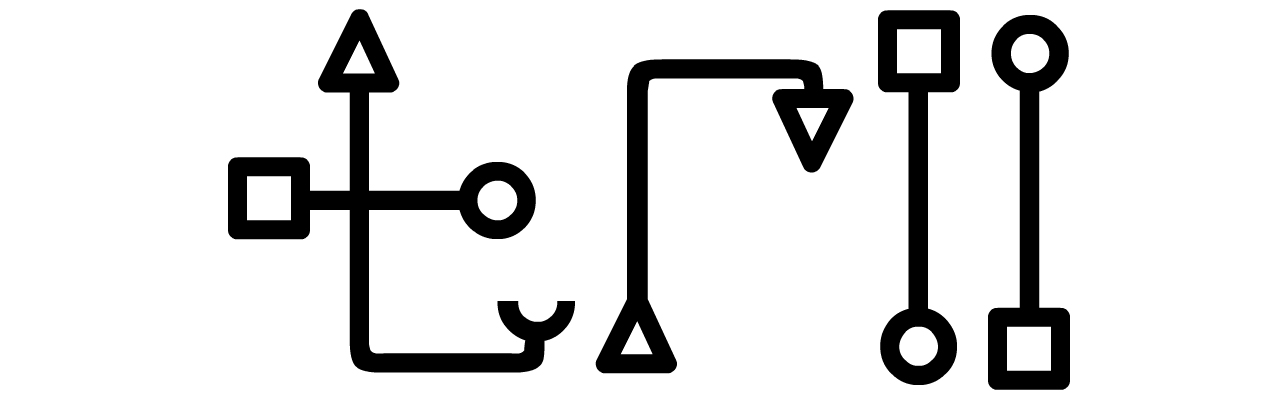
\includegraphics[width=5cm, height=1cm]{cos301logofinal.jpg}\\ 
	\textbf{Coding Standards Document}
	
	\noindent\makebox[\linewidth]{\rule{\paperwidth}{0.4pt}}\\ 
	\vspace*{100px}
	\textbf{Team Name: devs101} \\
	\textbf{Client Name: Mark-Anthony Fouch\'e}\\
		\vspace*{10px}
	\textbf{Team Members}\\
		\vspace*{3px}
		\begin{center}
      	\begin{itemize}
      	
      	\item Brendan Bath
      	\item Dylan Draper
      	\item Charles Claassen
      		\item Dail Nathan Jonker
      	\item Njaravani Christopher
        \end{itemize}
     \end{center}
     
     }
     \newpage
      \section{UML DIAGRAM }
     \section{Coding Conventions}
     \subsection{Naming Conventions}
     
     \subsubsection{Folder Names}
     \begin{itemize}
      	\item All folder names does start with a small letter and the name is descriptive enough to provide infromation on what exaclty they contain eg components, contains all components files
      	\end{itemize}
     \subsubsection{Class Names}
      	\begin{itemize}
      	\item All class names had to begin with capital letters and new name within the class name had to begin with capital letters aswell.
      	\end{itemize}
      	
    	  \subsubsection{Variables and Attributes} 
      \begin{itemize}
     	\item variableName - variables and attributes had to start with a lowercase letter and each new word within the same name had to begin with a Capital letter, meaning to say they have to be exactly the same 	as the methods.
     	\end{itemize}
     	\subsubsection{Accessors}
   \begin{itemize} 
 	 \item {\it eg getAttribute()} - had to follow the same rules as the methods and had to always be named after the variable which they intent to access.
 	 \end{itemize} 
 	 
  \subsubsection{Mutators}
   \begin{itemize} 
 	 \item eg setVariable(.....) - had to  follow the same naming conventions as methods i.e they had to start with a lowercase and any new name within the name should begin with a capital letter.
 	  \end{itemize} 
 	    \subsubsection{Packages} 
   \begin{itemize}
 	 \item eg display.package -  names of the packages had to  always be in lower-case letters and no 			upper-case.
 	 \end{itemize} 
 	 
   \subsubsection{File names}
    \begin{itemize} 
  		\item Vuetify.js - file names had to be descriptive enough to tell what they contain inside and name had to always 	begin with a small letter except only App.vue which loads initially which is like the main.eg rules.js shows that it contains rules, store.js thats the store file which stores files
	\end{itemize}
	\subsubsection{Exceptions}
 	\begin{itemize} 
 		\item Exceptions had to be applied and used wherever necessary and these should the following had to always be checked.
 		\item Exception classes had to be avoided if neccessary and more meaningful classes with meaningful names had to be used.No more functionality had to be in these classes except only catch 	statements so that they clearly show what exactly have happened without any confusion.
 		\item Appropriate catch statements had to be used which had to allow the program to continue if need be rather than crashing.
	\end{itemize}
	
	\subsubsection{Methods or Functions}
  \begin{itemize}
 	\item Methods had to be given a descriptive name of what exactly they do and the name had to begin with a lower-case letter and any new name 	within the name had to begin with a Capital letter for easier readability.
 	\end{itemize}  
 	
 	\subsection{Layout Rules}
 	\subsubsection{Indentation and Line spaces}
	\begin{itemize}
		\item Lines had to be kept of very small length so as to ensure readability.
		\item Once a line had reached  a certain length(mostly 8 words), it had to be broken 	and 				indented further than the previous line for readability.
		\item Indentation had  4 spaces for each level, blank lines to seperate methods and also to 				emphasize or make it clearer where each method ends.
		
		\item attributes had to be be defined mostly after the methods in a class.
		\item public final variables being the exception which had to be defined first.
	\end{itemize}
	
 	\subsection{Commenting Practises}
 		\begin{itemize}
		\item It was a mandatory to comments so that the code becomes very easy to read and understand
		\item Comments were added in blocks and not in lines as it might cause some confusion 						and the code wont be clean hence no readability.
		\item For line comments we used {\it // and multiline use /* ..*/}\\\\
		{\it for example int index  = 1; // index of starting point.}\\\\
		
		\end{itemize}
	\section{File Structure}
	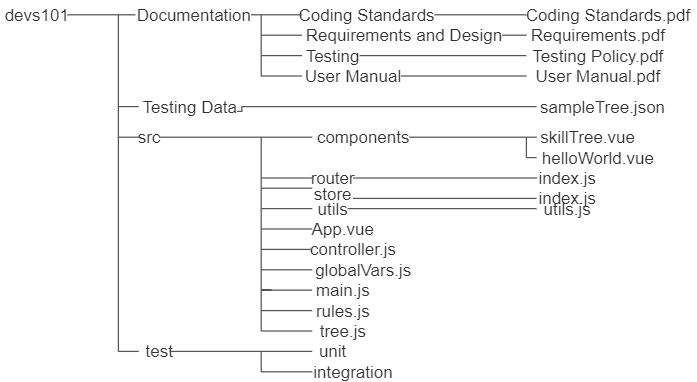
\includegraphics[width=15cm, height=10cm]{filestructure.jpg}\\ 
	
	\section{Code Review Process}
	\subsection{Pair Programming}
	\begin{itemize}
	\item Any 2 group volunteers will work in groups of two, code together, one coding while the other is 		reviewing the other's code.That follow up check made it sure that all coding standards rules are 			followed eg Variable naming conventions, bracketing and indentation
	\end{itemize}
	
	\subsection{Peer reviews}
	\begin{itemize}
	\item Any group member who get the chance can get to look at someone's code once the member is done.After each assignment of work, issues are created and before an issue is closed, that person's code shou
	\end{itemize}
\end{document}
